\documentclass[11pt]{article}
\usepackage[utf8]{inputenc}
\usepackage[T1]{fontenc}
\usepackage[spanish]{babel}
\usepackage{amsmath, amssymb, amsthm, mathtools}
\usepackage{braket}
\usepackage{dsfont}
\usepackage{graphicx}
\usepackage[margin=2.5cm]{geometry}
\usepackage{hyperref}
\emergencystretch=2em

\newcommand{\ii}{\mathrm{i}}
\newcommand{\ee}{\mathrm{e}}
\newcommand{\adag}{\hat a^\dagger}
\newcommand{\bdag}{\hat b^\dagger}
\newcommand{\sigmad}{\hat\sigma^\dagger}
\newcommand{\Tr}{\operatorname{Tr}}

\title{Modelo de Holstein-Cummings}
\author{Ricardo Del Rosal Gardu\~no \\ \small Doctorado en F\'isica, BUAP}
\date{Notas de doctorado: una mol\'ecula}

\begin{document}
\maketitle

\tableofcontents
\bigskip

\section{Idea f\'isica}

El modelo de Holstein-Cummings describe una mol\'ecula con tres grados de
libertad relevantes: una transici\'on electr\'onica efectiva de dos niveles, un
modo vibracional intramolecular y un modo cuantizado de cavidad. La idea
central es que la excitaci\'on electr\'onica no solo cambia la energ\'ia
interna de la mol\'ecula. Tambi\'en cambia la distribuci\'on electr\'onica y,
por eso, cambia la superficie de energ\'ia potencial que sienten los n\'ucleos.

En el estado electr\'onico base $\ket{g}$, la geometr\'ia nuclear de equilibrio
se toma como origen de una coordenada efectiva $q$. En el estado excitado
$\ket{e}$, la superficie sigue siendo aproximadamente arm\'onica, pero su
m\'inimo est\'a desplazado. Este desplazamiento produce el acoplamiento de
Holstein: el estado electr\'onico decide cu\'al es la posici\'on de equilibrio
del oscilador vibracional.

Para la tesis, este modelo es el punto de partida porque muestra c\'omo pasar
de una mol\'ecula aislada a una estructura por bloques que puede
diagonalizarse. La extensi\'on a dos mol\'eculas mantiene la misma l\'ogica,
pero el espacio de Hilbert crece y aparecen sectores donde la cavidad puede
mediar correlaciones entre mol\'eculas distintas.

\section{Superficies de energ\'ia potencial}

Se aproxima la vibraci\'on nuclear por un oscilador arm\'onico con masa
efectiva $m$ y frecuencia vibracional $\nu$. Si la mol\'ecula est\'a en el
estado electr\'onico base, se elige el m\'inimo en $q=0$:
\begin{equation}
  V_g(q)=\frac{1}{2}m\nu^2q^2.
\end{equation}
La coordenada $q$ mide la deformaci\'on respecto de la geometr\'ia de
equilibrio. Para una mol\'ecula diat\'omica puede tomarse como
$q=R-R_g$, donde $R$ es la distancia internuclear y $R_g$ la distancia de
equilibrio en el estado base. Si $q>0$, la mol\'ecula est\'a elongada; si
$q<0$, est\'a comprimida respecto de esa geometr\'ia.

En el estado electr\'onico excitado, la energ\'ia electr\'onica aumenta en
$\hbar\omega$ y el m\'inimo vibracional se desplaza a $q=q_0$:
\begin{equation}
  V_e(q)=\hbar\omega+\frac{1}{2}m\nu^2(q-q_0)^2.
\end{equation}
Si $q_0=0$, excitar la mol\'ecula no cambia su geometr\'ia de equilibrio y no
aparece acoplamiento electr\'onico-vibracional. Si $q_0\neq0$, la excitaci\'on
electr\'onica crea una fuerza efectiva sobre la coordenada nuclear.

\begin{figure}[htbp]
  \centering
  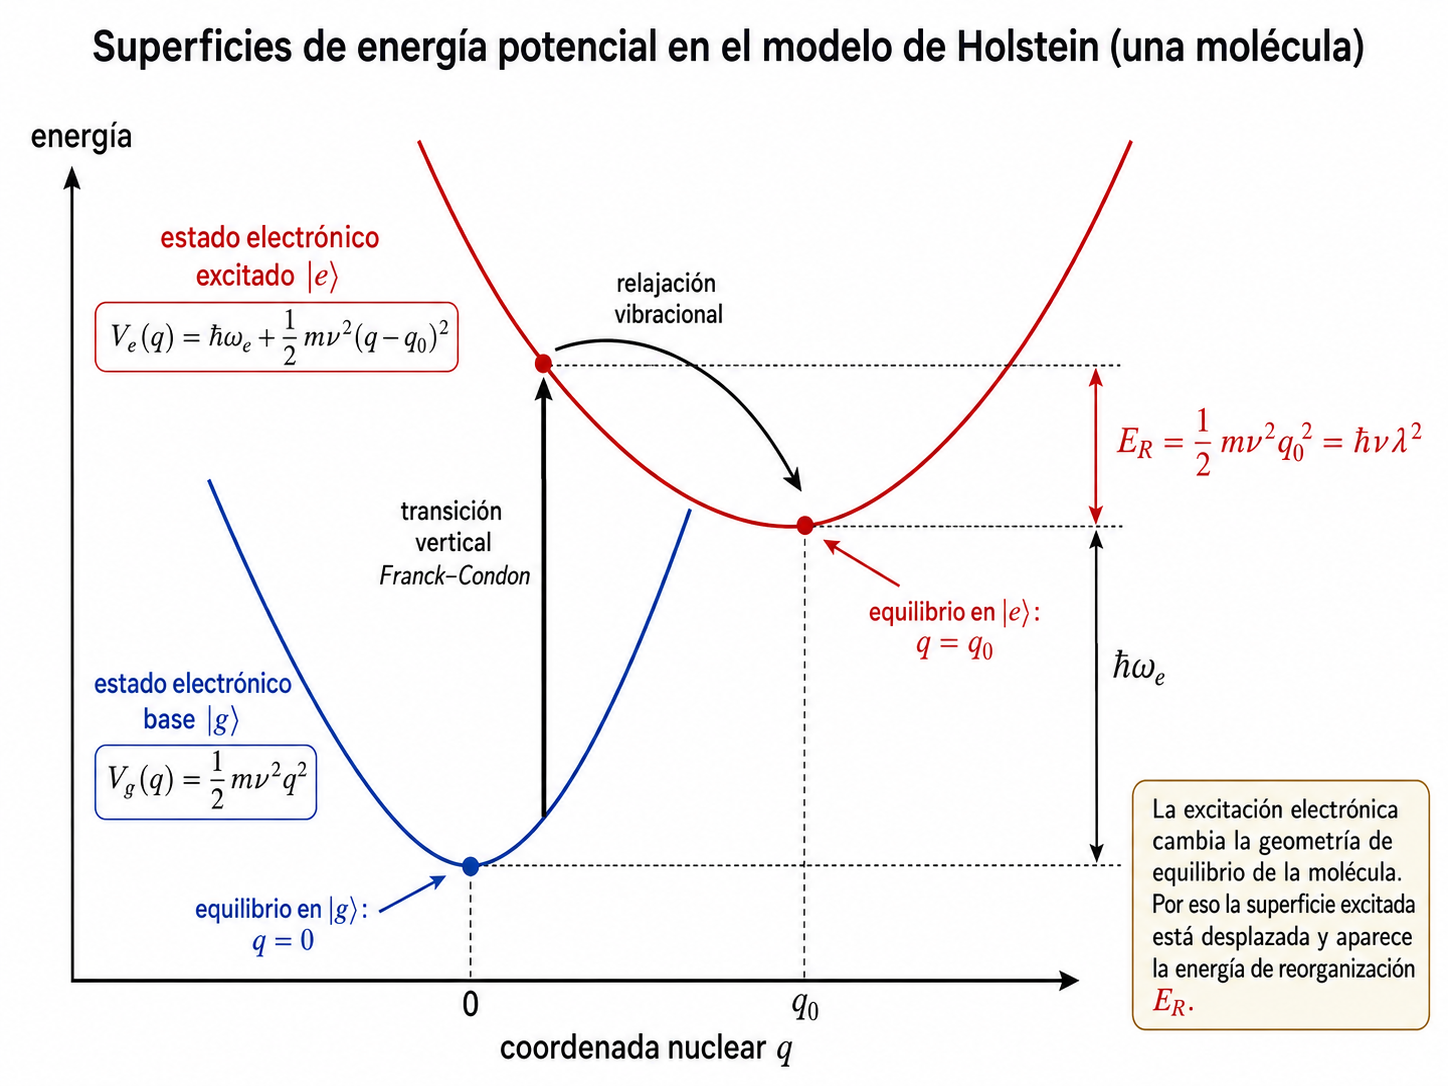
\includegraphics[width=0.95\linewidth]{../../notas-doctorado/imgs/superficies_de_energia.png}
  \caption{Superficies de energ\'ia potencial en el modelo de Holstein para
  una mol\'ecula. La transici\'on vertical de Franck-Condon ocurre antes de que
  los n\'ucleos puedan moverse, por eso la mol\'ecula queda inicialmente en
  $q=0$ sobre la superficie excitada.}
\end{figure}

La energ\'ia de reorganizaci\'on se obtiene comparando la energ\'ia de la
superficie excitada en $q=0$ con la energ\'ia en su m\'inimo $q=q_0$:
\begin{equation}
  V_e(0)=\hbar\omega+\frac{1}{2}m\nu^2q_0^2,
  \qquad
  V_e(q_0)=\hbar\omega.
\end{equation}
Por tanto,
\begin{equation}
  \boxed{
  E_R=V_e(0)-V_e(q_0)=\frac{1}{2}m\nu^2q_0^2.
  }
\end{equation}
Esta energ\'ia responde a una pregunta f\'isica concreta: despu\'es de excitar
electr\'onicamente la mol\'ecula sin mover los n\'ucleos todav\'ia, cu\'anta
energ\'ia puede liberar la mol\'ecula al relajar su geometr\'ia desde $q=0$
hasta $q=q_0$. Si $q_0$ es grande, la excitaci\'on deforma mucho la mol\'ecula
y $E_R$ es grande. Si $q_0=0$, ambas superficies tienen el mismo m\'inimo y
$E_R=0$.

La cantidad $\hbar\omega$ es la diferencia de energ\'ia entre m\'inimos. La
absorci\'on vertical de Franck-Condon desde $q=0$ hasta $q=0$ en la superficie
excitada cuesta
\begin{equation}
  V_e(0)-V_g(0)=\hbar\omega+E_R.
\end{equation}
Por eso la frecuencia efectiva de la transici\'on vertical se escribir\'a como
\begin{equation}
  \boxed{\omega_0=\omega+\nu\lambda^2}
\end{equation}
una vez que se introduzca el par\'ametro adimensional de Huang-Rhys
$\lambda$.

\section{Hamiltoniano molecular de Holstein}

Para una mol\'ecula aislada, el espacio de Hilbert se separa como
\begin{equation}
  \mathcal H_{\mathrm{mol}}
  =
  \mathcal H_{\mathrm{el}}\otimes\mathcal H_{\mathrm{vib}},
\end{equation}
donde $\mathcal H_{\mathrm{el}}$ est\'a generado por $\{\ket{g},\ket{e}\}$ y
$\mathcal H_{\mathrm{vib}}$ por los estados de n\'umero vibracionales
$\{\ket{m}_v\}_{m=0}^{\infty}$. Se definen los operadores electr\'onicos
\begin{equation}
  \sigmad=\ket{e}\bra{g},
  \qquad
  \hat\sigma=\ket{g}\bra{e},
  \qquad
  \sigmad\hat\sigma=\ket{e}\bra{e}.
\end{equation}
Tomando la energ\'ia electr\'onica del estado base como cero y la diferencia
entre m\'inimos como $\hbar\omega$, el hamiltoniano electr\'onico aislado es
\begin{equation}
  \hat H_{\mathrm{el}}
  =
  \hbar\omega\,\ket{e}\bra{e}
  =
  \hbar\omega\,\sigmad\hat\sigma.
\end{equation}

Al a\~nadir la vibraci\'on nuclear, el hamiltoniano vibracional condicionado
al estado electr\'onico es
\begin{equation}
  \hat H_{\mathrm{vib}}
  =
  \left[
  \frac{\hat p^2}{2m}
  +
  \frac{1}{2}m\nu^2\hat q^2
  \right]\ket{g}\bra{g}
  +
  \left[
  \frac{\hat p^2}{2m}
  +
  \frac{1}{2}m\nu^2(\hat q-q_0)^2
  \right]\ket{e}\bra{e}.
\end{equation}
Sumando la parte electr\'onica,
\begin{align}
  \hat H_{\mathrm{mol}}
  &=
  \left[
  \frac{\hat p^2}{2m}
  +
  \frac{1}{2}m\nu^2\hat q^2
  \right]\ket{g}\bra{g}
  \notag\\
  &\quad+
  \left[
  \hbar\omega
  +
  \frac{\hat p^2}{2m}
  +
  \frac{1}{2}m\nu^2(\hat q-q_0)^2
  \right]\ket{e}\bra{e}.
\end{align}
Al expandir $(\hat q-q_0)^2=\hat q^2+q_0^2-2q_0\hat q$ se obtiene
\begin{align}
  \hat H_{\mathrm{mol}}
  &=
  \left(
  \frac{\hat p^2}{2m}
  +
  \frac{1}{2}m\nu^2\hat q^2
  \right)\mathds{1}_{\mathrm{el}}
  +
  \hbar\omega\,\sigmad\hat\sigma
  \notag\\
  &\quad
  -m\nu^2q_0\hat q\,\sigmad\hat\sigma
  +
  \frac{1}{2}m\nu^2q_0^2\,\sigmad\hat\sigma .
\end{align}
Los t\'erminos tienen una lectura directa. El primero es la vibraci\'on
arm\'onica com\'un. El segundo es la energ\'ia electr\'onica. El tercero dice
que cuando la mol\'ecula est\'a excitada aparece una fuerza que desplaza la
coordenada nuclear. El \'ultimo es una constante energ\'etica asociada solo a
la superficie excitada.

Se cuantiza el oscilador vibracional con operadores bos\'onicos $\hat b$ y
$\bdag$ que satisfacen
\begin{equation}
  [\hat b,\bdag]=1,
  \qquad
  \bdag\ket{m}_v=\sqrt{m+1}\ket{m+1}_v,
  \qquad
  \hat b\ket{m}_v=\sqrt{m}\ket{m-1}_v .
\end{equation}
Las variables can\'onicas se escriben como
\begin{equation}
  \hat q=
  \sqrt{\frac{\hbar}{2m\nu}}\left(\bdag+\hat b\right),
  \qquad
  \hat p=
  \ii\sqrt{\frac{\hbar m\nu}{2}}\left(\bdag-\hat b\right).
\end{equation}
Sustituyendo estas expresiones,
\begin{align}
  \frac{\hat p^2}{2m}
  +
  \frac{1}{2}m\nu^2\hat q^2
  &=
  -\frac{\hbar\nu}{4}\left(\bdag-\hat b\right)^2
  +
  \frac{\hbar\nu}{4}\left(\bdag+\hat b\right)^2
  \notag\\
  &=
  \frac{\hbar\nu}{2}\left(\bdag\hat b+\hat b\bdag\right)
  \notag\\
  &=
  \hbar\nu\left(\bdag\hat b+\frac{1}{2}\right).
\end{align}
La energ\'ia de punto cero $\hbar\nu/2$ es constante y se descarta porque no
afecta la din\'amica.

El t\'ermino lineal se convierte en
\begin{equation}
  -m\nu^2q_0\hat q\,\sigmad\hat\sigma
  =
  -m\nu^2q_0
  \sqrt{\frac{\hbar}{2m\nu}}
  \left(\bdag+\hat b\right)\sigmad\hat\sigma .
\end{equation}
Se introduce el par\'ametro adimensional de Huang-Rhys:
\begin{equation}
  \boxed{
  \lambda^2=\frac{m\nu q_0^2}{2\hbar},
  \qquad
  \lambda=q_0\sqrt{\frac{m\nu}{2\hbar}}.
  }
\end{equation}
Con esta definici\'on,
\begin{equation}
  m\nu^2q_0\sqrt{\frac{\hbar}{2m\nu}}
  =
  \hbar\nu\lambda,
\end{equation}
y el t\'ermino de Holstein queda
\begin{equation}
  -\hbar\nu\lambda(\bdag+\hat b)\sigmad\hat\sigma .
\end{equation}
Adem\'as,
\begin{equation}
  \frac{1}{2}m\nu^2q_0^2=\hbar\nu\lambda^2,
\end{equation}
por lo que $E_R=\hbar\nu\lambda^2$. El hamiltoniano molecular toma la forma
\begin{equation}
  \boxed{
  \hat H_{\mathrm{mol}}
  =
  \hbar\omega_0\,\sigmad\hat\sigma
  +
  \hbar\nu\,\bdag\hat b
  -
  \hbar\nu\lambda(\bdag+\hat b)\sigmad\hat\sigma,
  \qquad
  \omega_0=\omega+\nu\lambda^2.
  }
\end{equation}

\section{Acoplamiento con la cavidad}

Para llegar al modelo de Holstein-Cummings se a\~nade un modo cuantizado de
cavidad. El espacio total es
\begin{equation}
  \mathcal H
  =
  \mathcal H_{\mathrm{cav}}
  \otimes
  \mathcal H_{\mathrm{el}}
  \otimes
  \mathcal H_{\mathrm{vib}},
\end{equation}
con base natural
\begin{equation}
  \ket{n}_c\otimes\ket{\alpha}\otimes\ket{m}_v,
  \qquad
  \alpha\in\{g,e\}.
\end{equation}
El hamiltoniano libre de cavidad, despu\'es de quitar su energ\'ia de punto
cero, es
\begin{equation}
  \hat H_{\mathrm{cav}}=\hbar\Omega\,\adag\hat a,
\end{equation}
donde $\Omega$ es la frecuencia del modo de cavidad y
$[\hat a,\adag]=1$. Si hay $n$ fotones,
$\adag\hat a\ket{n}_c=n\ket{n}_c$, y la energ\'ia fot\'onica es
$\hbar\Omega n$.

La mol\'ecula se acopla al campo mediante el momento dipolar de la transici\'on
electr\'onica. Aplicando la aproximaci\'on dipolar y la aproximaci\'on de onda
rotante al acoplamiento $-\hat{\mathbf d}\cdot\hat{\mathbf E}$, queda el
t\'ermino an\'alogo al de Jaynes-Cummings:
\begin{equation}
  \hat H_{\mathrm{int}}
  =
  \hbar g\left(\sigmad\hat a+\hat\sigma\adag\right).
\end{equation}
As\'i, el hamiltoniano de Holstein-Cummings para una sola mol\'ecula es
\begin{equation}
  \boxed{
  \hat H_{\mathrm{HC}}
  =
  \hbar\Omega\adag\hat a
  +
  \hbar\omega_0\sigmad\hat\sigma
  +
  \hbar\nu\bdag\hat b
  -
  \hbar\nu\lambda(\bdag+\hat b)\sigmad\hat\sigma
  +
  \hbar g\left(\sigmad\hat a+\hat\sigma\adag\right).
  }
\end{equation}
Este modelo acopla la transici\'on electr\'onica molecular con la vibraci\'on
y con la cavidad. No incluye un acoplamiento directo cavidad-vibraci\'on. Un
t\'ermino de ese tipo tendr\'ia la forma
\begin{equation}
  \hat H_{\mathrm{cav-vib}}
  =
  \hbar\eta(\hat a+\adag)(\hat b+\bdag)
  \simeq
  \hbar\eta(\hat a\bdag+\adag\hat b),
\end{equation}
despu\'es de una RWA apropiada. F\'isicamente no aparece porque la frecuencia
electr\'onica efectiva $\omega_0$ suele estar en el visible o ultravioleta,
mientras que la frecuencia vibracional $\nu$ suele estar en el infrarrojo. Un
\'unico modo de cavidad con frecuencia $\Omega$ no puede estar
simult\'aneamente en resonancia con $\omega_0$ y con $\nu$ en mol\'eculas
reales.

Si se pidiera $\Omega\simeq\omega_0\simeq\nu$, entonces
\begin{equation}
  \omega+\nu\lambda^2\simeq\nu
  \qquad\Rightarrow\qquad
  \lambda\simeq\sqrt{1-\frac{\omega}{\nu}}.
\end{equation}
Para que $\lambda$ sea real se requerir\'ia $\omega<\nu$, pero usualmente
$\omega\gg\nu$. Por eso no hay un par\'ametro real que haga resonantes, al
mismo tiempo, los tres subsistemas.

\section{Aproximaciones f\'isicas}

La construcci\'on anterior usa varias aproximaciones:
\begin{itemize}
  \item Aproximaci\'on de Born-Oppenheimer: las superficies electr\'onicas
  dependen de las coordenadas nucleares porque los n\'ucleos son mucho m\'as
  pesados que los electrones.
  \item Aproximaci\'on arm\'onica: cerca de cada m\'inimo, las superficies de
  energ\'ia potencial se aproximan por par\'abolas.
  \item Dos niveles electr\'onicos efectivos: aunque una mol\'ecula real tiene
  muchos estados electr\'onicos, se retiene una transici\'on dominante
  $\ket{g}\leftrightarrow\ket{e}$.
  \item Aproximaci\'on dipolar y RWA \'optica: el acoplamiento con la cavidad se
  reduce a $\hbar g(\sigmad\hat a+\hat\sigma\adag)$.
\end{itemize}

\section{Coordenada efectiva y modos vibracionales}

Para una mol\'ecula de $N_a$ \'atomos hay $3N_a$ coordenadas nucleares. Si la
mol\'ecula no es lineal, tres corresponden a traslaciones globales y tres a
rotaciones. Esas seis coordenadas no cambian la geometr\'ia interna, solo
mueven o giran la mol\'ecula completa. Por eso quedan $3N_a-6$ modos
vibracionales internos. Para una mol\'ecula lineal quedan $3N_a-5$, porque una
rotaci\'on alrededor del eje molecular no cambia la configuraci\'on.

En principio las superficies dependen de todas las coordenadas normales,
\begin{equation}
  V=V(Q_1,Q_2,\ldots,Q_{3N_a-6}).
\end{equation}
Si el proceso relevante ocurre principalmente a lo largo de una direcci\'on, se
introduce una coordenada de reacci\'on efectiva
\begin{equation}
  q=c_1Q_1+c_2Q_2+\cdots+c_{3N_a-6}Q_{3N_a-6}.
\end{equation}
Esta coordenada representa la combinaci\'on de desplazamientos nucleares que
m\'as se acopla a la transici\'on electr\'onica. Para una mol\'ecula diat\'omica,
puede coincidir con la distancia internuclear.

\section{N\'umero de excitaciones conservado}

Comparando con Jaynes-Cummings,
\begin{equation}
  \hat H_{\mathrm{JC}}
  =
  \hbar\Omega\adag\hat a
  +
  \frac{1}{2}\hbar\omega\,\hat\sigma_z
  +
  \hbar g(\sigmad\hat a+\hat\sigma\adag),
\end{equation}
se observa que el HC contiene el mismo intercambio resonante electr\'on-fot\'on,
pero a\~nade el modo vibracional y el acoplamiento de Holstein. Por eso se
pregunta si el n\'umero de excitaciones \'opticas
\begin{equation}
  \hat N=\adag\hat a+\sigmad\hat\sigma
\end{equation}
sigue siendo constante de movimiento. El t\'ermino vibracional
$\hbar\nu\bdag\hat b$ conmuta con $\hat N$ porque act\'ua en otro espacio de
Hilbert. El t\'ermino de Holstein tambi\'en conmuta con $\hat N$: contiene
$\bdag+\hat b$, que solo cambia fonones, y $\sigmad\hat\sigma$, que proyecta
sobre el estado excitado pero no cambia el n\'umero de excitaciones
electr\'onicas.
\begin{equation}
  \boxed{
  [\hat H_{\mathrm{HC}},\hat N]=0.
  }
\end{equation}
Los fonones no entran en $\hat N$ porque cambian el desplazamiento
vibracional, pero no crean ni destruyen excitaciones electr\'onicas ni fotones.
Esta conservaci\'on permite dividir el hamiltoniano en bloques de excitaci\'on
electr\'onica-fot\'onica fija.

\section{Bloques electr\'on-fot\'on}

Para $n\geq1$ excitaciones \'opticas, los estados electr\'on-fot\'on relevantes
son
\begin{equation}
  \ket{e,n-1},
  \qquad
  \ket{g,n},
\end{equation}
porque ambos tienen el mismo valor de $\hat N$. El primero tiene una
excitaci\'on electr\'onica y $n-1$ fotones, mientras que el segundo tiene cero
excitaciones electr\'onicas y $n$ fotones. El hamiltoniano no mezcla este
bloque con otro valor de $n$.

Se calcula la matriz de bloque en la base ordenada
$\{\ket{e,n-1},\ket{g,n}\}$, dejando los operadores vibracionales
$\hat b,\bdag$ sin diagonalizar. Los elementos diagonales son
\begin{align}
  \bra{e,n-1}\hat H_{\mathrm{HC}}\ket{e,n-1}
  &=
  \hbar
  \left[
  \Omega(n-1)+\omega_0+\nu\bdag\hat b
  -
  \nu\lambda(\bdag+\hat b)
  \right],
  \\
  \bra{g,n}\hat H_{\mathrm{HC}}\ket{g,n}
  &=
  \hbar\left[
  \Omega n+\nu\bdag\hat b
  \right].
\end{align}
La diferencia aparece porque solo la rama excitada $\ket{e,n-1}$ siente el
desplazamiento de Holstein. Los t\'erminos fuera de la diagonal provienen del
acoplamiento Cummings:
\begin{equation}
  \bra{e,n-1}\hat H_{\mathrm{HC}}\ket{g,n}
  =
  \bra{g,n}\hat H_{\mathrm{HC}}\ket{e,n-1}
  =
  \hbar g\sqrt n.
\end{equation}
Por tanto,
\begin{equation}
  \hat H_{\mathrm{HC}}^{(n)}
  =
  \hbar
  \begin{pmatrix}
  \Omega(n-1)+\omega_0+\nu\bdag\hat b-\nu\lambda(\bdag+\hat b)
  &
  g\sqrt n\\
  g\sqrt n
  &
  \Omega n+\nu\bdag\hat b
  \end{pmatrix}.
\end{equation}
Factorizando $\Omega n+\nu\bdag\hat b$, com\'un a la diagonal, y definiendo
\begin{equation}
  \Delta=\omega_0-\Omega,
\end{equation}
se obtiene
\begin{equation}
  \boxed{
  \hat H_{\mathrm{HC}}^{(n)}
  =
  \hbar\left(\Omega n+\nu\bdag\hat b\right)\mathds{1}_{2\times2}
  +
  \hbar
  \begin{pmatrix}
  \Delta-\nu\lambda(\bdag+\hat b) & g\sqrt n\\
  g\sqrt n & 0
  \end{pmatrix}.
  }
\end{equation}
Esta forma todav\'ia no es la forma sim\'etrica t\'ipica de un modelo de Rabi,
porque el acoplamiento vibracional aparece solo en la entrada superior.

\section{Desplazamiento vibracional del bloque}

Para manipular el bloque se introducen operadores auxiliares que act\'uan
dentro del subespacio $\{\ket{e,n-1},\ket{g,n}\}$:
\begin{equation}
  \hat\tau^{(n)\dagger}=\ket{e,n-1}\bra{g,n},
  \qquad
  \hat\tau^{(n)}=\ket{g,n}\bra{e,n-1},
\end{equation}
\begin{equation}
  \hat\tau_z^{(n)}
  =
  \ket{e,n-1}\bra{e,n-1}
  -
  \ket{g,n}\bra{g,n},
  \qquad
  \hat\tau_x^{(n)}
  =
  \hat\tau^{(n)\dagger}+\hat\tau^{(n)}.
\end{equation}
Estos operadores de subida y bajada no son los operadores electr\'onicos
f\'isicos $\sigmad$ y $\hat\sigma$. Cambian simult\'aneamente el estado
electr\'onico y el n\'umero de fotones para permanecer dentro del bloque $n$.

El proyector sobre la rama excitada del bloque es
\begin{equation}
  \hat P_e^{(n)}
  =
  \ket{e,n-1}\bra{e,n-1}
  =
  \frac{\mathds{1}_{2\times2}+\hat\tau_z^{(n)}}{2}.
\end{equation}
Con esto,
\begin{equation}
  \hat H_{\mathrm{HC}}^{(n)}
  =
  \hbar\left(\Omega n+\nu\bdag\hat b\right)\mathds{1}
  +
  \hbar\left[\Delta-\nu\lambda(\bdag+\hat b)\right]\hat P_e^{(n)}
  +
  \hbar g\sqrt n\,\hat\tau_x^{(n)}.
\end{equation}
Sustituyendo $\hat P_e^{(n)}$,
\begin{align}
  \hat H_{\mathrm{HC}}^{(n)}
  &=
  \hbar\left[
  \Omega n+\nu\bdag\hat b
  +
  \frac{\Delta}{2}
  -
  \frac{\nu\lambda}{2}(\hat b+\bdag)
  \right]\mathds{1}
  \notag\\
  &\quad
  +
  \frac{\hbar}{2}
  \left[
  \Delta-\nu\lambda(\hat b+\bdag)
  \right]\hat\tau_z^{(n)}
  +
  \hbar g\sqrt n\,\hat\tau_x^{(n)}.
\end{align}
El t\'ermino lineal proporcional a $\hat b+\bdag$ en la parte identidad
representa una fuerza uniforme sobre el oscilador vibracional. Se elimina
desplazando el origen del oscilador en el espacio de fase con
\begin{equation}
  \hat D(\alpha)=\ee^{\alpha\bdag-\alpha^*\hat b}.
\end{equation}
Para $\alpha$ real,
\begin{equation}
  \hat D^\dagger(\alpha)\hat b\,\hat D(\alpha)=\hat b+\alpha,
  \qquad
  \hat D^\dagger(\alpha)\bdag\,\hat D(\alpha)=\bdag+\alpha.
\end{equation}
Con $\alpha=\lambda/2$ se define
\begin{equation}
  \tilde H_{\mathrm{HC}}^{(n)}
  =
  \hat D^\dagger\!\left(\frac{\lambda}{2}\right)
  \hat H_{\mathrm{HC}}^{(n)}
  \hat D\!\left(\frac{\lambda}{2}\right).
\end{equation}
Esto equivale a sustituir
$\hat b\to\hat b+\lambda/2$ y $\bdag\to\bdag+\lambda/2$. Al hacerlo,
\begin{align}
  &\nu
  \left(\bdag+\frac{\lambda}{2}\right)
  \left(\hat b+\frac{\lambda}{2}\right)
  -
  \frac{\nu\lambda}{2}
  \left(\hat b+\bdag+\lambda\right)
  \notag\\
  &\qquad
  =
  \nu\bdag\hat b-\frac{\nu\lambda^2}{4}.
\end{align}
Por tanto,
\begin{align}
  \tilde H_{\mathrm{HC}}^{(n)}
  &=
  \hbar\left[
  \Omega n+\nu\bdag\hat b
  +
  \frac{\Delta}{2}
  -
  \frac{\nu\lambda^2}{4}
  \right]\mathds{1}
  \notag\\
  &\quad
  +
  \frac{\hbar}{2}
  \left[
  \Delta-\nu\lambda^2-\nu\lambda(\hat b+\bdag)
  \right]\hat\tau_z^{(n)}
  +
  \hbar g\sqrt n\,\hat\tau_x^{(n)}.
\end{align}
Se impone la condici\'on
\begin{equation}
  \Delta=\nu\lambda^2.
\end{equation}
Como $\Delta=\omega_0-\Omega$ y $\omega_0=\omega+\nu\lambda^2$, esta condici\'on
implica
\begin{equation}
  \omega+\nu\lambda^2-\Omega=\nu\lambda^2
  \qquad\Rightarrow\qquad
  \Omega=\omega.
\end{equation}
Es decir, la cavidad queda sintonizada con la transici\'on electr\'onica
natural entre m\'inimos, no con la transici\'on vertical $\omega_0$. Con esta
elecci\'on,
\begin{equation}
  \boxed{
  \tilde H_{\mathrm{HC}}^{(n)}
  =
  \hbar
  \left[
  \Omega n+\frac{\nu\lambda^2}{4}
  +
  \nu\bdag\hat b
  \right]\mathds{1}
  +
  \frac{\hbar}{2}
  \begin{pmatrix}
  -\nu\lambda(\hat b+\bdag) & 2g\sqrt n\\
  2g\sqrt n & \nu\lambda(\hat b+\bdag)
  \end{pmatrix}.
  }
\end{equation}

\section{Base polarit\'onica}

El t\'ermino Cummings que falta por diagonalizar es proporcional a
$\hat\tau_x^{(n)}$. Sus eigenestados son las combinaciones sim\'etrica y
antisim\'etrica:
\begin{equation}
  \boxed{
  \ket{\pm,n}
  =
  \frac{\ket{e,n-1}\pm\ket{g,n}}{\sqrt2}.
  }
\end{equation}
Estos son los polaritones del bloque resonante: ya no son mol\'ecula excitada
con $n-1$ fotones o mol\'ecula base con $n$ fotones por separado, sino
superposiciones coherentes de ambas posibilidades. En resonancia, cada
polarit\'on tiene mitad car\'acter material y mitad car\'acter fot\'onico.

En esta base se definen operadores de subida y bajada polarit\'onicos:
\begin{equation}
  \hat S^{(n)\dagger}=\ket{+,n}\bra{-,n},
  \qquad
  \hat S^{(n)}=\ket{-,n}\bra{+,n},
\end{equation}
\begin{equation}
  \hat S_z^{(n)}
  =
  \hat S^{(n)\dagger}\hat S^{(n)}
  -
  \hat S^{(n)}\hat S^{(n)\dagger},
  \qquad
  \hat S_x^{(n)}
  =
  \hat S^{(n)\dagger}+\hat S^{(n)}.
\end{equation}
Una cuenta directa da
\begin{equation}
  \hat S_z^{(n)}=\hat\tau_x^{(n)},
  \qquad
  \hat S_x^{(n)}=\hat\tau_z^{(n)}.
\end{equation}
Por eso el hamiltoniano desplazado se reescribe como
\begin{equation}
  \boxed{
  \tilde H_{\mathrm{HC}}^{(n)}
  =
  \hbar
  \left[
  \Omega n+\frac{\nu\lambda^2}{4}
  +
  \nu\bdag\hat b
  \right]\mathds{1}
  +
  \hbar g\sqrt n\,\hat S_z^{(n)}
  -
  \frac{\hbar\nu\lambda}{2}(\hat b+\bdag)\hat S_x^{(n)}.
  }
\end{equation}
En esta forma, cada bloque corresponde a un modelo de Rabi cu\'antico donde el
sistema de dos niveles efectivo no es la mol\'ecula desnuda, sino el doblete
polarit\'onico $\{\ket{+,n},\ket{-,n}\}$. El modo bos\'onico que se acopla a
ese pseudoesp\'in no es la cavidad, sino la vibraci\'on molecular.

\section{JCP efectivo polarit\'on-fon\'on}

El acoplamiento polarit\'on-vibraci\'on se expande como
\begin{align}
  (\hat b+\bdag)\hat S_x^{(n)}
  &=
  (\hat b+\bdag)
  \left(\hat S^{(n)\dagger}+\hat S^{(n)}\right)
  \notag\\
  &=
  \hat b\hat S^{(n)\dagger}
  +
  \bdag\hat S^{(n)}
  +
  \hat b\hat S^{(n)}
  +
  \bdag\hat S^{(n)\dagger}.
\end{align}
Los primeros dos t\'erminos conservan energ\'ia cerca de la resonancia
polarit\'on-fon\'on: $\hat b\hat S^{(n)\dagger}$ destruye un fon\'on y sube el
polarit\'on, mientras que $\bdag\hat S^{(n)}$ crea un fon\'on y baja el
polarit\'on. Los otros dos t\'erminos son contra-rotantes: bajan ambos
subsistemas o suben ambos subsistemas simult\'aneamente.

Aplicando una RWA an\'aloga a la de Jaynes-Cummings se obtiene
\begin{equation}
  \boxed{
  \tilde H_{\mathrm{ef}}^{(n)}
  =
  \hbar
  \left[
  \Omega n+\frac{\nu\lambda^2}{4}
  +
  \nu\bdag\hat b
  \right]\mathds{1}
  +
  \hbar g\sqrt n\,\hat S_z^{(n)}
  -
  \frac{\hbar\nu\lambda}{2}
  \left(
  \hat b\hat S^{(n)\dagger}
  +
  \bdag\hat S^{(n)}
  \right).
  }
\end{equation}
Este hamiltoniano es del tipo Jaynes-Cummings-Paul, pero ahora el modo
bos\'onico es el fon\'on y el pseudo\'atomo es el doblete polarit\'onico.

La constante de movimiento del hamiltoniano efectivo es el n\'umero
polarit\'on-fon\'on
\begin{equation}
  \boxed{
  \hat M^{(n)}
  =
  \bdag\hat b+\hat S^{(n)\dagger}\hat S^{(n)},
  \qquad
  [\tilde H_{\mathrm{ef}}^{(n)},\hat M^{(n)}]=0.
  }
\end{equation}
Esto ocurre porque $\hat b\hat S^{(n)\dagger}$ destruye un fon\'on y sube el
polarit\'on, mientras que $\bdag\hat S^{(n)}$ crea un fon\'on y baja el
polarit\'on. En ambos casos, la suma total se conserva.

\section{Diagonalizaci\'on de dobletes}

Para $m>0$, la base relevante con n\'umero $\hat M^{(n)}=m$ es
\begin{equation}
  \ket{+,n,m-1},
  \qquad
  \ket{-,n,m}.
\end{equation}
El primer estado tiene $m-1$ fonones y una excitaci\'on polarit\'onica
superior. El segundo tiene $m$ fonones y el polarit\'on inferior. Ambos tienen
el mismo valor de $\hat M^{(n)}$.

Se usan las acciones
\begin{equation}
  \hat S_z^{(n)}\ket{+,n,m}=+\ket{+,n,m},
  \qquad
  \hat S_z^{(n)}\ket{-,n,m}=-\ket{-,n,m},
\end{equation}
\begin{equation}
  \hat S^{(n)\dagger}\ket{-,n,m}=\ket{+,n,m},
  \qquad
  \hat S^{(n)}\ket{+,n,m}=\ket{-,n,m},
\end{equation}
\begin{equation}
  \bdag\ket{\pm,n,m}=\sqrt{m+1}\ket{\pm,n,m+1},
  \qquad
  \hat b\ket{\pm,n,m}=\sqrt m\,\ket{\pm,n,m-1}.
\end{equation}
Los elementos diagonales son
\begin{align}
  \bra{+,n,m-1}\tilde H_{\mathrm{ef}}^{(n)}
  \ket{+,n,m-1}
  &=
  \hbar
  \left[
  \Omega n+\frac{\nu\lambda^2}{4}
  +
  \nu(m-1)
  +
  g\sqrt n
  \right],
  \\
  \bra{-,n,m}\tilde H_{\mathrm{ef}}^{(n)}
  \ket{-,n,m}
  &=
  \hbar
  \left[
  \Omega n+\frac{\nu\lambda^2}{4}
  +
  \nu m
  -
  g\sqrt n
  \right].
\end{align}
Los t\'erminos fuera de la diagonal provienen de
$-\hbar\nu\lambda(\hat b\hat S^\dagger+\bdag\hat S)/2$:
\begin{equation}
  \bra{+,n,m-1}\tilde H_{\mathrm{ef}}^{(n)}
  \ket{-,n,m}
  =
  \bra{-,n,m}\tilde H_{\mathrm{ef}}^{(n)}
  \ket{+,n,m-1}
  =
  -\frac{\hbar\nu\lambda}{2}\sqrt m.
\end{equation}
As\'i, en la base ordenada $\{\ket{+,n,m-1},\ket{-,n,m}\}$,
\begin{equation}
  \tilde H_{\mathrm{ef}}^{(n,m)}
  =
  \hbar
  \begin{pmatrix}
  \Omega n+\frac{\nu\lambda^2}{4}+\nu(m-1)+g\sqrt n
  &
  -\frac{\nu\lambda}{2}\sqrt m\\
  -\frac{\nu\lambda}{2}\sqrt m
  &
  \Omega n+\frac{\nu\lambda^2}{4}+\nu m-g\sqrt n
  \end{pmatrix}.
\end{equation}
El promedio de la diagonal es
\begin{equation}
  A_{nm}
  =
  \Omega n+\frac{\nu\lambda^2}{4}
  +
  \nu\left(m-\frac{1}{2}\right),
\end{equation}
y la diferencia entre las dos entradas diagonales es
\begin{equation}
  2g\sqrt n-\nu.
\end{equation}
Se define la desintonizaci\'on polarit\'on-fon\'on
\begin{equation}
  \delta_n=2g\sqrt n-\nu.
\end{equation}
Entonces
\begin{equation}
  \boxed{
  \tilde H_{\mathrm{ef}}^{(n,m)}
  =
  \hbar A_{nm}\mathds{1}_{2\times2}
  +
  \frac{\hbar}{2}
  \begin{pmatrix}
  \delta_n & -\nu\lambda\sqrt m\\
  -\nu\lambda\sqrt m & -\delta_n
  \end{pmatrix}.
  }
\end{equation}
La resonancia efectiva ocurre cuando
\begin{equation}
  \delta_n=0
  \qquad\Rightarrow\qquad
  \nu=2g\sqrt n,
\end{equation}
es decir, cuando la separaci\'on entre los polaritones del bloque $n$ coincide
con la frecuencia vibracional.

Para simplificar la diagonalizaci\'on se define
\begin{equation}
  k_m=\nu\lambda\sqrt m.
\end{equation}
Entonces el hamiltoniano del doblete puede escribirse como
\begin{equation}
  \tilde H_{\mathrm{ef}}^{(n,m)}
  =
  \hbar A_{nm}\mathds{1}_{2\times2}
  +
  \frac{\hbar}{2}
  \begin{pmatrix}
  \delta_n & -k_m\\
  -k_m & -\delta_n
  \end{pmatrix}.
\end{equation}
El primer t\'ermino suma la misma energ\'ia a los dos estados del doblete. Al
ser proporcional a la identidad, desplaza los eigenvalores pero no modifica los
eigenvectores. Por eso basta con diagonalizar la matriz del segundo t\'ermino.

Para diagonalizar la parte no trivial se resuelve
\begin{equation}
  \det
  \begin{pmatrix}
  \delta_n-\epsilon & -k_m\\
  -k_m & -\delta_n-\epsilon
  \end{pmatrix}
  =
  0.
\end{equation}
Esto da
\begin{equation}
  -(\delta_n^2-\epsilon^2)-k_m^2=0
  \qquad\Rightarrow\qquad
  \epsilon^2=\delta_n^2+k_m^2.
\end{equation}
Se define la frecuencia de Rabi efectiva del doblete $(n,m)$:
\begin{equation}
  \boxed{
  \Omega_{nm}^{\mathrm{ef}}
  =
  \sqrt{\delta_n^2+k_m^2}
  =
  \sqrt{\delta_n^2+\nu^2\lambda^2m}
  =
  \sqrt{(2g\sqrt n-\nu)^2+\nu^2\lambda^2m}.
  }
\end{equation}
Los eigenvalores son
\begin{equation}
  \boxed{
  E_{nm}^{\pm}
  =
  \hbar
  \left[
  \Omega n+\frac{\nu\lambda^2}{4}
  +
  \nu\left(m-\frac{1}{2}\right)
  \pm
  \frac{1}{2}\Omega_{nm}^{\mathrm{ef}}
  \right].
  }
\end{equation}
Para obtener los eigenvectores se trabaja con la parte no trivial
\begin{equation}
  M_{nm}
  =
  \begin{pmatrix}
  \delta_n & -k_m\\
  -k_m & -\delta_n
  \end{pmatrix},
\end{equation}
porque el t\'ermino $\hbar A_{nm}\mathds{1}_{2\times2}$ solo desplaza la
energ\'ia. En la base ordenada $\{\ket{+,n,m-1},\ket{-,n,m}\}$, un vector
arbitrario se escribe como
\begin{equation}
  \ket{u}
  =
  u\ket{+,n,m-1}
  +
  v\ket{-,n,m}
  \qquad\Longleftrightarrow\qquad
  \begin{pmatrix}
  u\\
  v
  \end{pmatrix}.
\end{equation}
Primero se toma el eigenvalor positivo de $M_{nm}$,
$\epsilon=+\Omega_{nm}^{\mathrm{ef}}$. Entonces
\begin{equation}
  \begin{pmatrix}
  \delta_n & -k_m\\
  -k_m & -\delta_n
  \end{pmatrix}
  \begin{pmatrix}
  u\\
  v
  \end{pmatrix}
  =
  \Omega_{nm}^{\mathrm{ef}}
  \begin{pmatrix}
  u\\
  v
  \end{pmatrix}.
\end{equation}
Multiplicando la matriz se obtiene el sistema
\begin{equation}
  u\delta_n-vk_m=\Omega_{nm}^{\mathrm{ef}}u,
  \qquad
  -uk_m-v\delta_n=\Omega_{nm}^{\mathrm{ef}}v.
\end{equation}
De la primera ecuaci\'on,
\begin{equation}
  -vk_m=(\Omega_{nm}^{\mathrm{ef}}-\delta_n)u
  \qquad\Rightarrow\qquad
  -\frac{v}{u}
  =
  \frac{\Omega_{nm}^{\mathrm{ef}}-\delta_n}{k_m}.
\end{equation}
Se elige entonces
\begin{equation}
  u=C_{nm},
  \qquad
  v=-S_{nm},
\end{equation}
con lo cual
\begin{equation}
  \ket{E_{nm}^{+}}
  =
  C_{nm}\ket{+,n,m-1}
  -
  S_{nm}\ket{-,n,m},
  \qquad
  \frac{S_{nm}}{C_{nm}}
  =
  \frac{\Omega_{nm}^{\mathrm{ef}}-\delta_n}{k_m}.
\end{equation}
Para normalizar se impone $\braket{E_{nm}^{+}|E_{nm}^{+}}=1$. Como la base es
ortonormal, resulta
\begin{equation}
  C_{nm}^2+S_{nm}^2=1.
\end{equation}
Tomando $C_{nm},S_{nm}\in\mathbb{R}^{+}$ y definiendo
$r=S_{nm}/C_{nm}$, se tiene
\begin{equation}
  C_{nm}^2+S_{nm}^2
  =
  C_{nm}^2+C_{nm}^2r^2
  =
  C_{nm}^2(1+r^2)
  =
  1,
\end{equation}
por lo que
\begin{equation}
  C_{nm}^2=\frac{1}{1+r^2}.
\end{equation}
Adem\'as,
\begin{equation}
  (\Omega_{nm}^{\mathrm{ef}})^2=\delta_n^2+k_m^2
  \qquad\Rightarrow\qquad
  k_m^2
  =
  (\Omega_{nm}^{\mathrm{ef}})^2-\delta_n^2
  =
  (\Omega_{nm}^{\mathrm{ef}}-\delta_n)
  (\Omega_{nm}^{\mathrm{ef}}+\delta_n).
\end{equation}
Por tanto,
\begin{equation}
  r^2
  =
  \left(
  \frac{\Omega_{nm}^{\mathrm{ef}}-\delta_n}{k_m}
  \right)^2
  =
  \frac{\Omega_{nm}^{\mathrm{ef}}-\delta_n}
  {\Omega_{nm}^{\mathrm{ef}}+\delta_n}.
\end{equation}
Al sustituir este resultado en la normalizaci\'on,
\begin{equation}
  C_{nm}^2
  =
  \frac{1}
  {1+\dfrac{\Omega_{nm}^{\mathrm{ef}}-\delta_n}
  {\Omega_{nm}^{\mathrm{ef}}+\delta_n}}
  =
  \frac{\Omega_{nm}^{\mathrm{ef}}+\delta_n}
  {2\Omega_{nm}^{\mathrm{ef}}},
\end{equation}
y por consiguiente
\begin{equation}
  S_{nm}^2
  =
  1-C_{nm}^2
  =
  \frac{\Omega_{nm}^{\mathrm{ef}}-\delta_n}
  {2\Omega_{nm}^{\mathrm{ef}}}.
\end{equation}
As\'i,
\begin{equation}
  C_{nm}
  =
  \sqrt{
  \frac{\Omega_{nm}^{\mathrm{ef}}+\delta_n}
  {2\Omega_{nm}^{\mathrm{ef}}}
  },
  \qquad
  S_{nm}
  =
  \sqrt{
  \frac{\Omega_{nm}^{\mathrm{ef}}-\delta_n}
  {2\Omega_{nm}^{\mathrm{ef}}}
  }.
\end{equation}
Para el eigenvalor negativo, $\epsilon=-\Omega_{nm}^{\mathrm{ef}}$, se tiene
\begin{equation}
  \begin{pmatrix}
  \delta_n & -k_m\\
  -k_m & -\delta_n
  \end{pmatrix}
  \begin{pmatrix}
  u\\
  v
  \end{pmatrix}
  =
  -\Omega_{nm}^{\mathrm{ef}}
  \begin{pmatrix}
  u\\
  v
  \end{pmatrix}.
\end{equation}
De nuevo, al multiplicar la matriz,
\begin{equation}
  u\delta_n-vk_m=-\Omega_{nm}^{\mathrm{ef}}u,
  \qquad
  -uk_m-v\delta_n=-\Omega_{nm}^{\mathrm{ef}}v.
\end{equation}
De la segunda ecuaci\'on se obtiene
\begin{equation}
  uk_m=(\Omega_{nm}^{\mathrm{ef}}-\delta_n)v
  \qquad\Rightarrow\qquad
  \frac{u}{v}
  =
  \frac{\Omega_{nm}^{\mathrm{ef}}-\delta_n}{k_m}.
\end{equation}
Por eso se escoge
\begin{equation}
  u=S_{nm},
  \qquad
  v=C_{nm},
\end{equation}
y el eigenvector negativo queda
\begin{equation}
  \ket{E_{nm}^{-}}
  =
  S_{nm}\ket{+,n,m-1}
  +
  C_{nm}\ket{-,n,m}.
\end{equation}
De esta forma los dos eigenvectores son ortogonales:
\begin{equation}
  \braket{E_{nm}^{+}|E_{nm}^{-}}
  =
  C_{nm}S_{nm}-S_{nm}C_{nm}
  =
  0.
\end{equation}
Ahora se construye el \'angulo de mezcla. Como
\begin{equation}
  (\Omega_{nm}^{\mathrm{ef}})^2=\delta_n^2+k_m^2
  \qquad\Rightarrow\qquad
  1
  =
  \left(
  \frac{\delta_n}{\Omega_{nm}^{\mathrm{ef}}}
  \right)^2
  +
  \left(
  \frac{k_m}{\Omega_{nm}^{\mathrm{ef}}}
  \right)^2,
\end{equation}
se puede definir
\begin{equation}
  \cos\theta_{nm}
  =
  \frac{\delta_n}{\Omega_{nm}^{\mathrm{ef}}},
  \qquad
  \sin\theta_{nm}
  =
  \frac{k_m}{\Omega_{nm}^{\mathrm{ef}}}
  =
  \frac{\nu\lambda\sqrt m}{\Omega_{nm}^{\mathrm{ef}}}.
\end{equation}
Con estas dos relaciones se fija el cuadrante del \'angulo. En particular,
cuando la raz\'on est\'a bien definida,
\begin{equation}
  \tan\theta_{nm}=\frac{k_m}{\delta_n}.
\end{equation}
Las identidades de medio \'angulo dan
\begin{equation}
  \cos^2\left(\frac{\theta_{nm}}{2}\right)
  =
  \frac{1+\cos\theta_{nm}}{2}
  =
  \frac{1}{2}
  \left(
  1+\frac{\delta_n}{\Omega_{nm}^{\mathrm{ef}}}
  \right)
  =
  \frac{\Omega_{nm}^{\mathrm{ef}}+\delta_n}
  {2\Omega_{nm}^{\mathrm{ef}}},
\end{equation}
\begin{equation}
  \sin^2\left(\frac{\theta_{nm}}{2}\right)
  =
  \frac{1-\cos\theta_{nm}}{2}
  =
  \frac{1}{2}
  \left(
  1-\frac{\delta_n}{\Omega_{nm}^{\mathrm{ef}}}
  \right)
  =
  \frac{\Omega_{nm}^{\mathrm{ef}}-\delta_n}
  {2\Omega_{nm}^{\mathrm{ef}}}.
\end{equation}
Comparando con las constantes de normalizaci\'on,
\begin{equation}
  C_{nm}
  =
  \cos\left(\frac{\theta_{nm}}{2}\right),
  \qquad
  S_{nm}
  =
  \sin\left(\frac{\theta_{nm}}{2}\right).
\end{equation}
De esta manera, los eigenvectores son
\begin{equation}
  \boxed{
  \ket{E_{nm}^{+}}
  =
  \cos\left(\frac{\theta_{nm}}{2}\right)\ket{+,n,m-1}
  -
  \sin\left(\frac{\theta_{nm}}{2}\right)\ket{-,n,m},
  }
\end{equation}
\begin{equation}
  \boxed{
  \ket{E_{nm}^{-}}
  =
  \sin\left(\frac{\theta_{nm}}{2}\right)\ket{+,n,m-1}
  +
  \cos\left(\frac{\theta_{nm}}{2}\right)\ket{-,n,m}.
  }
\end{equation}
Si $\delta_n=0$, entonces $\theta_{nm}=\pi/2$ y los eigenestados son
superposiciones equilibradas de $\ket{+,n,m-1}$ y $\ket{-,n,m}$. Por otro lado,
si $|\delta_n|\gg |k_m|$, el acoplamiento mezcla d\'ebilmente los dos estados.
En particular, para $\delta_n>0$ se tiene $\theta_{nm}\ll1$ y los eigenestados
se parecen mucho a los estados desnudos de la base efectiva.

\section{Sectores del modelo}

La base diagonal del hamiltoniano efectivo se organiza en tres sectores.

\subsection{Sector \texorpdfstring{$n=0$}{n=0}}

Si $n=0$, no hay fotones en el campo y la mol\'ecula est\'a en el estado base.
El \'unico estado electr\'on-fot\'on posible es $\ket{g,0}$, porque
$\ket{e,-1}$ requerir\'ia un n\'umero negativo de fotones. Los estados de este
sector son
\begin{equation}
  \ket{g,0,m},
  \qquad
  m=0,1,2,\ldots.
\end{equation}
En este caso solo contribuye la energ\'ia vibracional:
\begin{equation}
  \boxed{
  E_{g,0,m}=\hbar\nu m.
  }
\end{equation}

\subsection{Sector \texorpdfstring{$n>0$, $m=0$}{n mayor que cero, m=0}}

Si $n>0$ pero $m=0$, no existe el estado $\ket{+,n,-1}$ porque tendr\'ia
$-1$ fonones. Solo queda $\ket{-,n,0}$. Este sector es un bloque
unidimensional con energ\'ia
\begin{equation}
  \boxed{
  E_{n,0}^{-}
  =
  \hbar\left(\Omega n+\frac{\nu\lambda^2}{4}-g\sqrt n\right).
  }
\end{equation}
Este estado tiene el modo vibracional en el vac\'io.

\subsection{Sector din\'amico \texorpdfstring{$n>0$, $m>0$}{n mayor que cero, m mayor que cero}}

Este es el sector verdaderamente din\'amico. Para cada par $(n,m)$ hay dos
estados con el mismo n\'umero polarit\'on-fon\'on:
\begin{equation}
  \ket{+,n,m-1},
  \qquad
  \ket{-,n,m}.
\end{equation}
El primer estado tiene $m-1$ fonones y una excitaci\'on polarit\'onica
superior; el segundo tiene $m$ fonones y el polarit\'on inferior. La interacci\'on
efectiva produce oscilaciones coherentes entre un fon\'on vibracional y una
excitaci\'on polarit\'onica. Si $\delta_n=0$, ambos estados est\'an en
resonancia y se mezclan fuertemente. Si $|\delta_n|$ es grande comparado con
$\nu|\lambda|\sqrt m$, la mezcla es d\'ebil.

En este sector los eigenestados son $\ket{E_{nm}^{\pm}}$ y las energ\'ias son
$E_{nm}^{\pm}$.

\section{Validez del modelo efectivo}

Los pasos que llevan del hamiltoniano HC original al hamiltoniano efectivo
$\tilde H_{\mathrm{ef}}^{(n,m)}$ requieren varias condiciones f\'isicas.

Primero, el acoplamiento vibracional efectivo debe ser d\'ebil frente a la
frecuencia vibracional:
\begin{equation}
  \nu\gg\frac{\nu|\lambda|}{2}
  \qquad\Rightarrow\qquad
  |\lambda|\ll2.
\end{equation}
Esto impide que el desplazamiento entre superficies sea tan grande que los
t\'erminos contra-rotantes del modelo de Rabi fon\'onico se vuelvan importantes.
Como $\lambda^2$ es el factor de Huang-Rhys, esta condici\'on corresponde a un
r\'egimen vibro-electr\'onico d\'ebil o moderado.

Segundo, debe cumplirse la resonancia fon\'on-polarit\'on:
\begin{equation}
  \nu\simeq2g\sqrt n
  \qquad\Rightarrow\qquad
  \delta_n\simeq0.
\end{equation}
Despu\'es de pasar a polaritones, la separaci\'on energ\'etica entre
$\ket{+,n}$ y $\ket{-,n}$ es $2\hbar g\sqrt n$. Para que el fon\'on intercambie
energ\'ia de manera eficiente con el pseudoesp\'in polarit\'onico, su
frecuencia debe coincidir aproximadamente con esa separaci\'on.

Tercero, se impuso
\begin{equation}
  \Delta=\nu\lambda^2,
  \qquad
  \Delta=\omega_0-\Omega,
  \qquad
  \omega_0=\omega+\nu\lambda^2.
\end{equation}
Por tanto,
\begin{equation}
  \Omega=\omega.
\end{equation}
F\'isicamente, la cavidad queda sintonizada con la transici\'on electr\'onica
natural entre m\'inimos. Esta condici\'on elimina el t\'ermino est\'atico
residual que quedar\'ia en el pseudoesp\'in despu\'es del desplazamiento.

Un conjunto t\'ipico de escalas, tomando $g$ como unidad, puede organizarse
como
\begin{equation}
  \Omega=1000g,
  \qquad
  \nu=\alpha g,
  \qquad
  \nu\lambda\simeq0.01g,
  \qquad
  \omega_0=\Omega+\nu\lambda^2.
\end{equation}
De $\nu\lambda\simeq0.01g$ se sigue
\begin{equation}
  \alpha g\,\lambda\simeq0.01g
  \qquad\Rightarrow\qquad
  \lambda^2\simeq\frac{10^{-4}}{\alpha^2}.
\end{equation}
La energ\'ia de reorganizaci\'on es entonces
\begin{equation}
  \nu\lambda^2\simeq\frac{10^{-4}}{\alpha}g.
\end{equation}
La resonancia fon\'on-polarit\'on exige $\alpha\simeq2\sqrt n$. Para $n=1$,
$\alpha\simeq2$, de modo que $\lambda\simeq0.005$ y
\begin{equation}
  \nu\lambda^2\simeq5\times10^{-5}g.
\end{equation}
Estas escalas son f\'isicamente posibles, aunque describen un acoplamiento
vibro-electr\'onico extremadamente d\'ebil.

La conclusi\'on de validez es
\begin{equation}
  \boxed{
  \Omega,\omega,\omega_0\gg g,\nu,\nu|\lambda|.
  }
\end{equation}
La escala \'optica debe ser mucho m\'as r\'apida que la din\'amica efectiva
polarit\'on-fon\'on.

\section{Valores esperados}

La diagonalizaci\'on se hizo en un espacio desplazado. Si
\begin{equation}
  \ket{\tilde\Psi(t)}
  =
  \hat D^\dagger\!\left(\frac{\lambda}{2}\right)
  \ket{\Psi(t)},
\end{equation}
entonces cualquier valor esperado f\'isico debe calcularse como
\begin{equation}
  \boxed{
  \langle\hat O\rangle
  =
  \bra{\Psi(t)}\hat O\ket{\Psi(t)}
  =
  \bra{\tilde\Psi(t)}
  \hat D^\dagger\!\left(\frac{\lambda}{2}\right)
  \hat O
  \hat D\!\left(\frac{\lambda}{2}\right)
  \ket{\tilde\Psi(t)}.
  }
\end{equation}
Si $\hat O$ act\'ua solo en el espacio electr\'onico o fot\'onico, conmuta con
$\hat D(\lambda/2)$ porque el desplazamiento act\'ua \'unicamente sobre el
modo vibracional. En ese caso, el valor esperado es igual en el espacio
f\'isico y en el espacio desplazado.

Si $\hat O$ depende de $\hat b$, $\bdag$, $\hat q$, $\hat p$ o
$\bdag\hat b$, entonces el operador s\'i debe transformarse. Por ejemplo,
\begin{equation}
  \hat D^\dagger\!\left(\frac{\lambda}{2}\right)
  \hat b\,
  \hat D\!\left(\frac{\lambda}{2}\right)
  =
  \hat b+\frac{\lambda}{2},
\end{equation}
\begin{equation}
  \hat D^\dagger\!\left(\frac{\lambda}{2}\right)
  \bdag\hat b\,
  \hat D\!\left(\frac{\lambda}{2}\right)
  =
  \left(\bdag+\frac{\lambda}{2}\right)
  \left(\hat b+\frac{\lambda}{2}\right).
\end{equation}
Solo los observables que no ven el desplazamiento son invariantes.

\section{Conexi\'on con la tesis}

El resultado central de esta nota es que el hamiltoniano de Holstein-Cummings
para una mol\'ecula puede reducirse, bajo condiciones f\'isicas claras, a
dobletes efectivos del tipo Jaynes-Cummings-Paul entre polaritones y fonones.
La diagonalizaci\'on ocurre en dos niveles. Primero se forman polaritones a
partir de la mezcla coherente entre mol\'ecula y cavidad. Despu\'es, el
acoplamiento de Holstein mezcla esos polaritones con el modo vibracional.

Para dos mol\'eculas, la estrategia natural ser\'a conservar esta
organizaci\'on: construir el hamiltoniano completo, identificar el n\'umero de
excitaciones \'opticas conservado, elegir una base por sectores y analizar
c\'omo los modos vibracionales intramoleculares modifican la estructura
polarit\'onica. La dificultad nueva es que habr\'a m\'as ramas electr\'onicas y
m\'as caminos de intercambio mediado por la cavidad. El caso de una mol\'ecula
fija la notaci\'on y el criterio f\'isico para no perderse en esa extensi\'on.

\bigskip

El modelo HC muestra que la vibraci\'on molecular no se acopla directamente a
la cavidad. Entra al problema porque el car\'acter electr\'onico de los
polaritones hereda el desplazamiento de Holstein. Esa es la pieza que se debe
rastrear con cuidado al pasar de una mol\'ecula a dos.

\end{document}
